
\newacronym{rbf}{RBF}{Radial Basis Function}
\newacronym{kpca-s}{KPCA-S}{Kernel PCA with Sigmoid kernel}
\newacronym{kpca-r}{KPCA-R}{Kernel PCA with RBF kernel}
\section{Experiment 3}
This experiment is targetted towards \gls{pca} and \gls{kpca}. The goal is to compare the performance of \gls{pca} and \gls{kpca}, because these methods are similar, with the exception that \gls{kpca} implements a kernel. Beause of the similarity of the methods, comparison will be more focused on the impact the different kernels can have on the model, namely what numbers does the machine learning model confuse given the different kernels.


As explained in the Chapter Theory, KPCA can have kernels, which will project the data into a higher dimensional feature space, where a hyperplane can be constructed, and perform PCA on it. KPCA does not require the transformation of the inputs into the feature space with the kernel function, but can use the kernels so as to get the dot product of the pair-wise input points~\cite{kpca-book}.


The kernels are a measure of similarity between the points~\cite{scikit-learn}, which means that points that are close to each other have higher similarity score, which is computed with the kernel function. The kernels chosen for the experiment are the \gls{rbf} and sigmoid kernels. The sigmoid kernel \textcquote{scikit-learn}{computes the sigmoid kernel between two vectors}, which outputs a value between -1 and 1 for the two given input vectors. The \gls{rbf} kernel \textcquote{scikit-learn}{computes the radial basis function kernel between two vectors}, which outputs a value between 0 and 1.


\subsection{Rules}
This experiment will not use gridsearch. The input of the data samples will be 15000 for both of the methods, because of hardware limitations. The amount of components used for the methods will be the ones that were used in experiment one, namely 49 components. The evaluation will be based on the confusion matrices, and eventually also for the score of the methods. The kernels used will be \gls{rbf} and sigmoid.


\subsection{Results}
Figure \ref{fig:confusion-matrix-pca-svm} shows the results for \gls{pca}.
Figure~\ref{fig:confusion-matrix-kernel-pca-svm-sigmoid} shows the results for \gls{kpca} with sigmoid kernel.
Figure~\ref{fig:confusion-matrix-kernel-pca-svm-rbf} shows the results for \gls{kpca} with rbf kernel.


\begin{figure}[htb!]
    \centering
    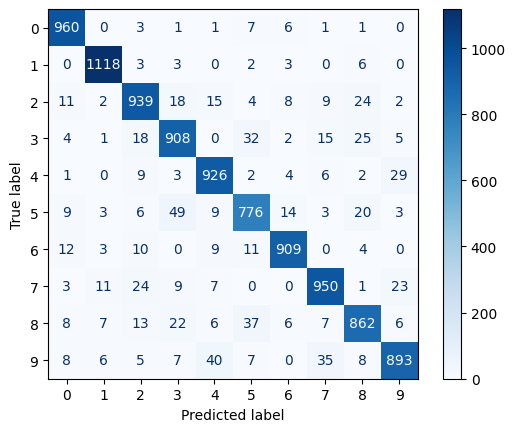
\includegraphics[width=0.5\textwidth]{../src/results/experiment_three/confusion_matrix_pca_svm.png}
    \caption{Confusion matrix for PCA}
    \label{fig:confusion-matrix-pca-svm}
\end{figure}





\begin{figure}
    \centering
    \subfloat[\centering Confusion matrix for kPCA Sigmoid]{\label{fig:confusion-matrix-kernel-pca-svm-sigmoid}{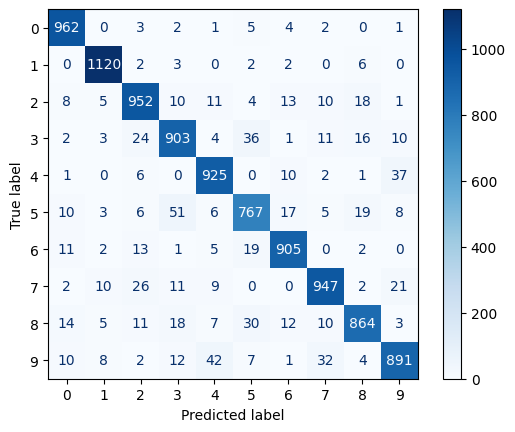
\includegraphics[width=0.45\textwidth]{../src/results/experiment_three/confusion_matrix_kernel_pca_svm_sigmoid.png} }}
    \qquad
    \subfloat[\centering Confusion matrix for kPCA RBF]{\label{fig:confusion-matrix-kernel-pca-svm-rbf}{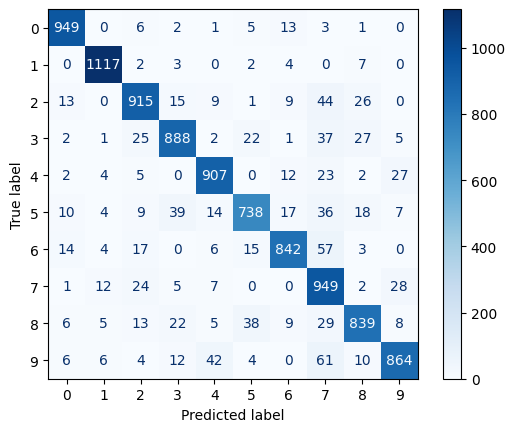
\includegraphics[width=0.45\textwidth]{../src/results/experiment_three/kernel_pca_rbf_kernel_49.png} }}%
    \caption{both kPCA kernels confusion matrices}
    \label{fig:kpca-kernels}
\end{figure}






\subsection{Results}
A slight improvement over the number 0 has been seen in \gls{kpca-s} in that it mapped 11 numbers better than \gls{pca}, and the same can be said for the number 2.

Both methods acquired the same amount of correct predictions for the numbers 3 and 4.

A slight difference appears in the number 5, where \gls{pca} has 780 correct predictions, and \gls{kpca-s} got 767, which is worse than \gls{pca}. The reason for that is because it confused it with the numbers 3 and 6.


A slight improvement in \gls{kpca-s} is seen at the number 6, where it got five numbers more than \gls{pca}. Such a low number is not worth considering, however.

It can be seen that sigmoid confuses the number 7 with the number 9 more often than \gls{pca} normally would, which worsens \gls{kpca-s}' ability to predict the number 7 correctly.

The notable impressions regarding the differences between \gls{pca} and \gls{kpca-s} are: \gls{kpca-s} improved by about ten numbers at the numbers 0 and 2, became worse at the number 5, became worse at the number 7, and shined the most at the number 8. The most interesting cases are the numbers 0,2, 5, and 8.


The RBF kernel has confused more number 2's than any other method presented in this experiment. As opposed to \gls{pca} and \gls{kpca-s}, \gls{kpca-r} confused it 33 times more with the number 7 and around ten times more with the number 8. The same pattern can be seen at the number 3, where it was again confused with numbers 7 and 8.


\gls{kpca-r} has confused the number 4 mainly with the numbers 7 and 9, and \gls{kpca-s} has only confused it with the number 9. Concerning the number 4, \gls{kpca-s} is the only method that has confused it the most with the number 9.


\gls{kpca-r} mainly confuses the number 5 with the numbers 3 and 7, whereas \gls{kpca-s} does it with the numbers 3, 6, and 8, and the same can be said about \gls{pca}.

The number 6 reveals a potentially interesting finding: \gls{kpca-r} is the only method that managed to confuse the number 6 with the number 7, as opposed to the other methods, which did not confuse it with the number 7.

The only place where \gls{kpca-r} outshines \gls{kpca-s} is at the number 7, where \gls{kpca-r} confuses with two numbers less than \gls{kpca-s}. Such a finding, however, is not of major importance because \gls{kpca-r} underperforms most of the time. 

\subsubsection{Summary of the differences between the methods}
From the results presented so far about the differences between the kernels it can be seen that all the methods often confuse the number 2 with 8; 3 with 2,5,8 and to a certain degree(PCA and much worse with \gls{kpca-r}), 7. The methods also confuse the number 4 with 9; 5 with 3,6, and 8 (\gls{kpca-r} also does it with 7). The number 6 gets confused with the number 0,2,5 (\gls{kpca-r} also does it with 7).
The number 7 gets confused with the number 2,3 and 9. \gls{kpca-r} is the only one that did not confuse the number 3 as much as the other methods.

At number 8, the methods have confused 0 (except for \gls{kpca-r}),2,3 and 5. \gls{kpca-r} confused it again with the number 7, but it is the only one that managed to map the number 0 less than the other methods. Lastly the number 9 got confused with the numbers the most with the numbers 4 and 7. It can be further noted that \gls{kpca-r} is the worst at confusing various numbers with the number 7.


From the overview provided regarding the difference in numbers, a percentage would be more preferable, more specifically, a percentage of the errors made in the numbers 0-9. Table \ref{tab:error-percentage-pca-kpca-s-kpca-r} shows the difference in percentages of errors made by the methods for each number.

\begin{table}[htb!]
    \centering
    \begin{tabular}{lrrrr}
        \toprule
          & pca    & kpca-s & kpca-r \\
        \midrule
        0 & 2.959  & 1.836  & 3.163  \\
        1 & 1.585  & 1.321  & 1.585  \\
        2 & 8.817  & 7.751  & 11.337 \\
        3 & 10.594 & 10.594 & 12.079 \\
        4 & 5.702  & 5.804  & 7.637  \\
        5 & 12.556 & 14.013 & 17.264 \\
        6 & 6.054  & 5.532  & 12.108 \\
        7 & 7.101  & 7.879  & 7.684  \\
        8 & 13.552 & 11.293 & 13.860 \\
        9 & 11.992 & 11.694 & 14.370 \\
        \bottomrule
    \end{tabular}
    \caption{Error percentage for each number for the methods}
    \label{tab:error-percentage-pca-kpca-s-kpca-r}
\end{table}

Another finding which could be explored is the difference in the number of errors made by the methods for each number. Table \ref{tab:error-percentage-pca-kpca-s-kpca-r} shows the difference in the number of errors made by the methods for each number.

Yet another finding that could be explored is to research why \gls{kpca-r} is the only method that confuses many numbers with the number 7.
%\subsection{Discussion of results}

